% =====================================================================
%  Presentación final · Procesos de ramificación en complejos celulares
%  Simulación Estocástica · Primavera 2026
%
%  PLAN DE TIEMPOS (~9:15, pareja; cada persona habla >= 3 min)
%    Bloque 1 · El proyecto y por qué importa ........ ~3:00  (Persona 1)
%    Bloque 2 · Resultados ............................ ~4:15  (Persona 1 hasta "Cargas
%                                                               conservadas", luego Persona 2)
%    Bloque 3 · Conclusiones y pasos futuros ......... ~2:00  (Persona 2, cierra con Ninja)
%    => Persona 1 ~4:30, Persona 2 ~4:45
%  Después del "¡Gracias!" hay diapositivas de RESPALDO para las preguntas.
%  Pauta: 25% globalidad y tiempos · 35% avances · 25% audiovisual · 15% oral
%
%  Las líneas "% GUION:" son lo que se dice; NO aparecen en las diapositivas.
%  Videos: los enlaces "ver video" abren el MP4 en GitHub (tenerlos abiertos aparte).
% =====================================================================
\documentclass[aspectratio=169,11pt]{beamer}

\usetheme[progressbar=frametitle, numbering=fraction, sectionpage=progressbar]{metropolis}
\usepackage[T1]{fontenc}
\usepackage[utf8]{inputenc}
\usepackage[spanish,es-noshorthands,es-nodecimaldot,es-tabla]{babel}
\usepackage{amsmath,amssymb,mathtools}
\usepackage{booktabs}
\usepackage{tikz}
\usetikzlibrary{arrows.meta}
\graphicspath{{figuras/}}

% ---------------------------------------------------------------------
%  Paleta "café con dulce de leche"
% ---------------------------------------------------------------------
\definecolor{cafe}{HTML}{3E271C}        % café oscuro: títulos y texto
\definecolor{cafeleche}{HTML}{7A543A}   % café con leche: bloques
\definecolor{dulce}{HTML}{C4864A}       % dulce de leche: acentos
\definecolor{dulceosc}{HTML}{A0642C}    % dulce de leche tostado: texto destacado
\definecolor{caramelo}{HTML}{E2B683}    % caramelo claro: barra de progreso
\definecolor{leche}{HTML}{F3E6D3}       % leche: fondo de bloques
\definecolor{crema}{HTML}{FBF6EE}       % crema: fondo de las diapositivas
% partículas, igual que en los videos
\definecolor{rojo}{RGB}{214,39,40}
\definecolor{azul}{RGB}{33,102,194}
\definecolor{verde}{HTML}{8FD18F}

\setbeamercolor{normal text}{fg=cafe, bg=crema}
\setbeamercolor{background canvas}{bg=crema}
\setbeamercolor{frametitle}{fg=crema, bg=cafe}
\setbeamercolor{palette primary}{fg=crema, bg=cafe}          % diapositivas standout
\setbeamercolor{progress bar}{fg=dulce, bg=caramelo}
\setbeamercolor{title separator}{fg=dulce}
\setbeamercolor{progress bar in head/foot}{fg=dulce, bg=caramelo}
\setbeamercolor{progress bar in section page}{fg=dulce, bg=caramelo}
\setbeamercolor{alerted text}{fg=dulceosc}
\setbeamercolor{example text}{fg=cafeleche}
\setbeamercolor{block title}{fg=crema, bg=cafeleche}
\setbeamercolor{block body}{fg=cafe, bg=leche}
\setbeamercolor{block title alerted}{fg=crema, bg=dulceosc}
\setbeamercolor{block body alerted}{fg=cafe, bg=leche}
\setbeamercolor{itemize item}{fg=dulce}
\setbeamercolor{enumerate item}{fg=dulce}

\newcommand{\Z}{\mathbb{Z}}
\DeclareMathOperator{\sgn}{sgn}
\newcommand{\ip}[2]{\langle #1,#2\rangle}
\newcommand{\repo}{https://github.com/martinmaturana777/Branching-Process-Complexes}
\newcommand{\video}[2]{\href{\repo/blob/main/videos/#1}{\small\textcolor{dulceosc}{$\blacktriangleright$ #2}}}

\title{Procesos de ramificación en complejos celulares}
\subtitle{Simulación, extinción y conjuntos absorbentes}
\author{Martín Maturana Acevedo \and Bruno Guevara}
\institute{\scriptsize Simulación Estocástica · Universidad de Chile · basado en \emph{Branching process on complexes}, D.~Cid y A.~Sepúlveda}
\date{Noviembre 2026}

\begin{document}

% =====================================================================
%  BLOQUE 1 · EL PROYECTO Y POR QUÉ IMPORTA · ~3:00 · Persona 1
% =====================================================================

% --- Portada con collage de cuadros de los videos ---
\begin{frame}[plain]
  % GUION (0:15): presentarse; "simulamos un proceso de partículas que vive en las aristas de una grilla".
  \begin{tikzpicture}[remember picture, overlay]
    \fill[crema] (current page.south west) rectangle (current page.north east);
    \fill[cafe] (current page.south west) rectangle ([yshift=0.3cm]current page.south east);
    \node[anchor=north east, inner sep=0] at ([xshift=-0.35cm, yshift=-0.35cm]current page.north east)
      {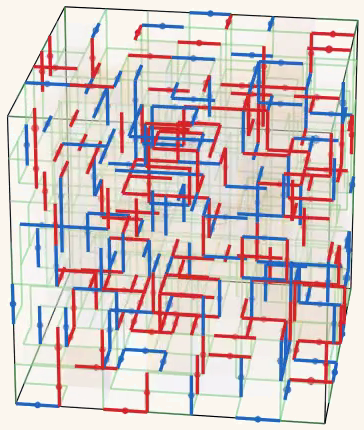
\includegraphics[height=4.9cm]{portada_3d}};
    \node[anchor=south east, inner sep=0] at ([xshift=-3.75cm, yshift=0.55cm]current page.south east)
      {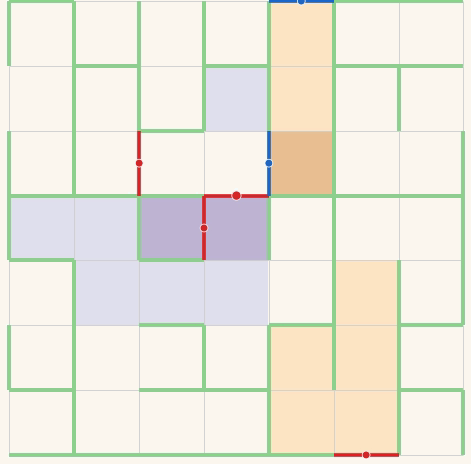
\includegraphics[height=2.9cm]{portada_2d}};
    \node[anchor=south east, inner sep=0] at ([xshift=-0.35cm, yshift=0.55cm]current page.south east)
      {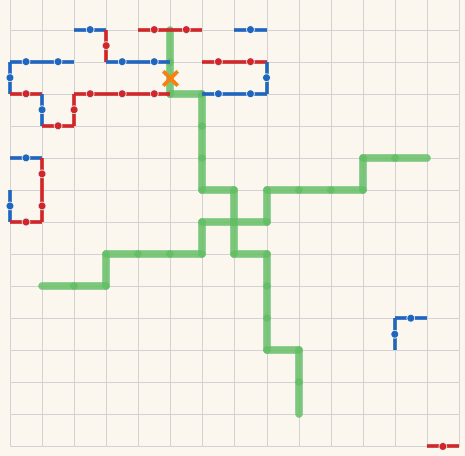
\includegraphics[height=2.9cm]{portada_ninja}};
    \node[anchor=north west, text width=7.4cm, align=left, inner sep=0] at ([xshift=0.7cm, yshift=-1.1cm]current page.north west) {%
      {\LARGE\bfseries\color{cafe} Procesos de ramificación\\[1mm] en complejos celulares}\\[3mm]
      {\color{dulceosc} Simulación, extinción y\\ conjuntos absorbentes}\\[2mm]
      {\color{dulce}\rule{6cm}{1.2pt}}\\[3mm]
      {\color{cafe} Martín Maturana Acevedo\\ Bruno Guevara}\\[2mm]
      {\footnotesize\color{cafeleche} Simulación Estocástica · Universidad de Chile\\ Noviembre 2026}\\[1.5mm]
      {\scriptsize\color{cafeleche} Basado en \emph{Branching process on complexes}\\ de D.~Cid y A.~Sepúlveda}};
  \end{tikzpicture}
\end{frame}

\metroset{sectionpage=none}
\section{El proyecto}

\begin{frame}{De los grafos a los complejos}
  % GUION (0:20): un paseo aleatorio vive en vértices; aquí las partículas viven en aristas
  % y tienen carga (+ rojo, - azul). Las que interactúan son las caras (cuadraditos).
  % La regla: cuando una cara "suena" se le resta su borde. Lo vemos en acción ->
  \centering
  \begin{tikzpicture}[scale=1.3]
    \foreach \x in {0,...,4} \draw[cafe!25] (\x,0) -- (\x,3);
    \foreach \y in {0,...,3} \draw[cafe!25] (0,\y) -- (4,\y);
    \fill[leche] (1.05,1.05) rectangle (1.95,1.95); \node at (1.5,1.5) {$f$};
    \draw[very thick, rojo] (1,1) -- (2,1); \fill[rojo] (1.5,1) circle (2.2pt);
    \draw[very thick, azul] (3,1) -- (3,2); \fill[azul] (3,1.5) circle (2.2pt);
    \draw[very thick, rojo] (0,2) -- (0,3); \fill[rojo] (0,2.5) circle (2.2pt);
  \end{tikzpicture}
  \vspace{4mm}

  $\theta\in\Z^{E}$: \textcolor{rojo}{partículas $+$} y \textcolor{azul}{partículas $-$} sobre las aristas\\[2mm]
  $\theta\;\longmapsto\;\theta-\ip{e}{\partial f}\sgn(\theta_e)\,\partial f$
\end{frame}

\begin{frame}{El proceso: estado inicial}
  % GUION (~1:00 para las 7 diapositivas): en cada evento (1) suena el reloj de una
  % partícula, (2) elige una cara vecina y cada arista del borde recibe ±1, (3) se resta
  % el borde: la partícula muere y nacen otras; ✕ = aniquilación (+ con -), ○ = absorbida
  % por el árbol verde. Simulación real (caja 4×4); se eligió la primera semilla en que los
  % 2 eventos muestran ramificación, aniquilación y absorción (presentacion/animacion_proceso.py).
  \centering
  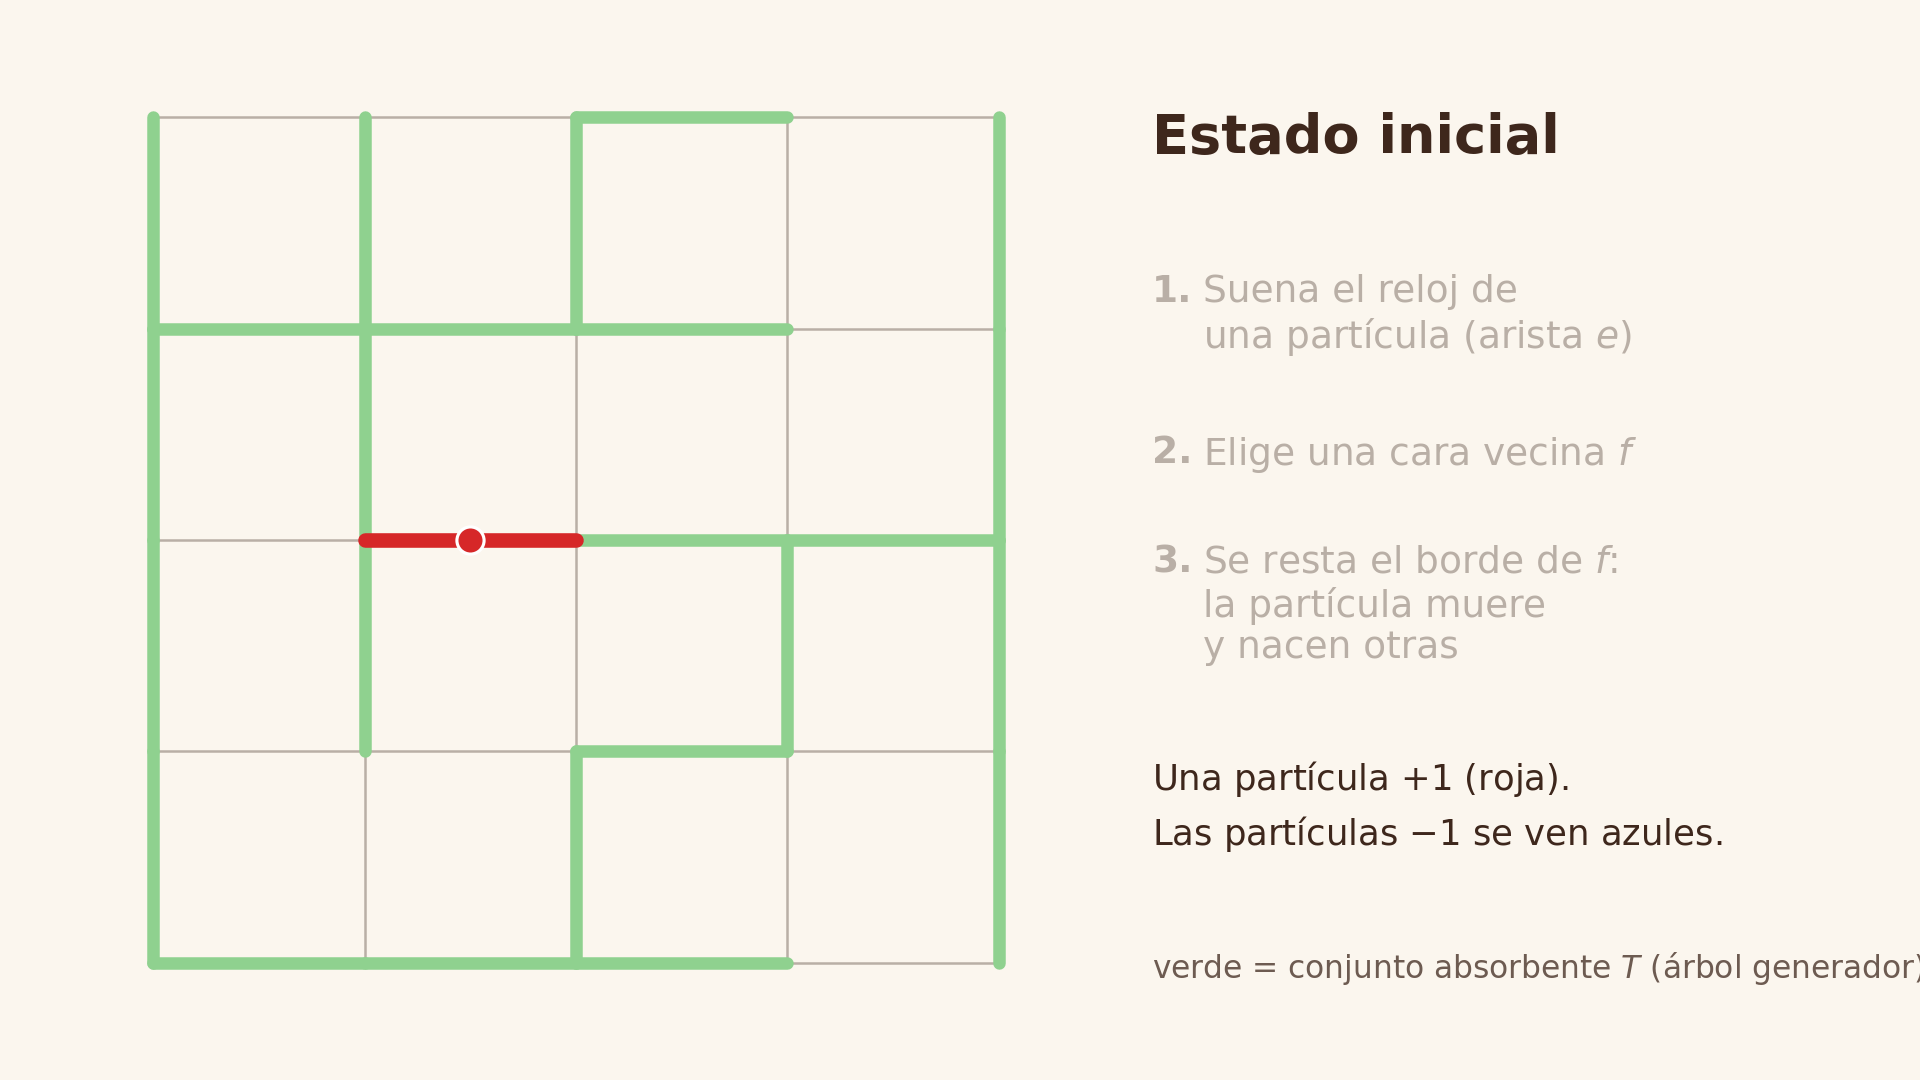
\includegraphics[height=0.84\textheight]{proceso/paso_00}
\end{frame}

\begin{frame}{Evento 1 · suena un reloj}
  \centering
  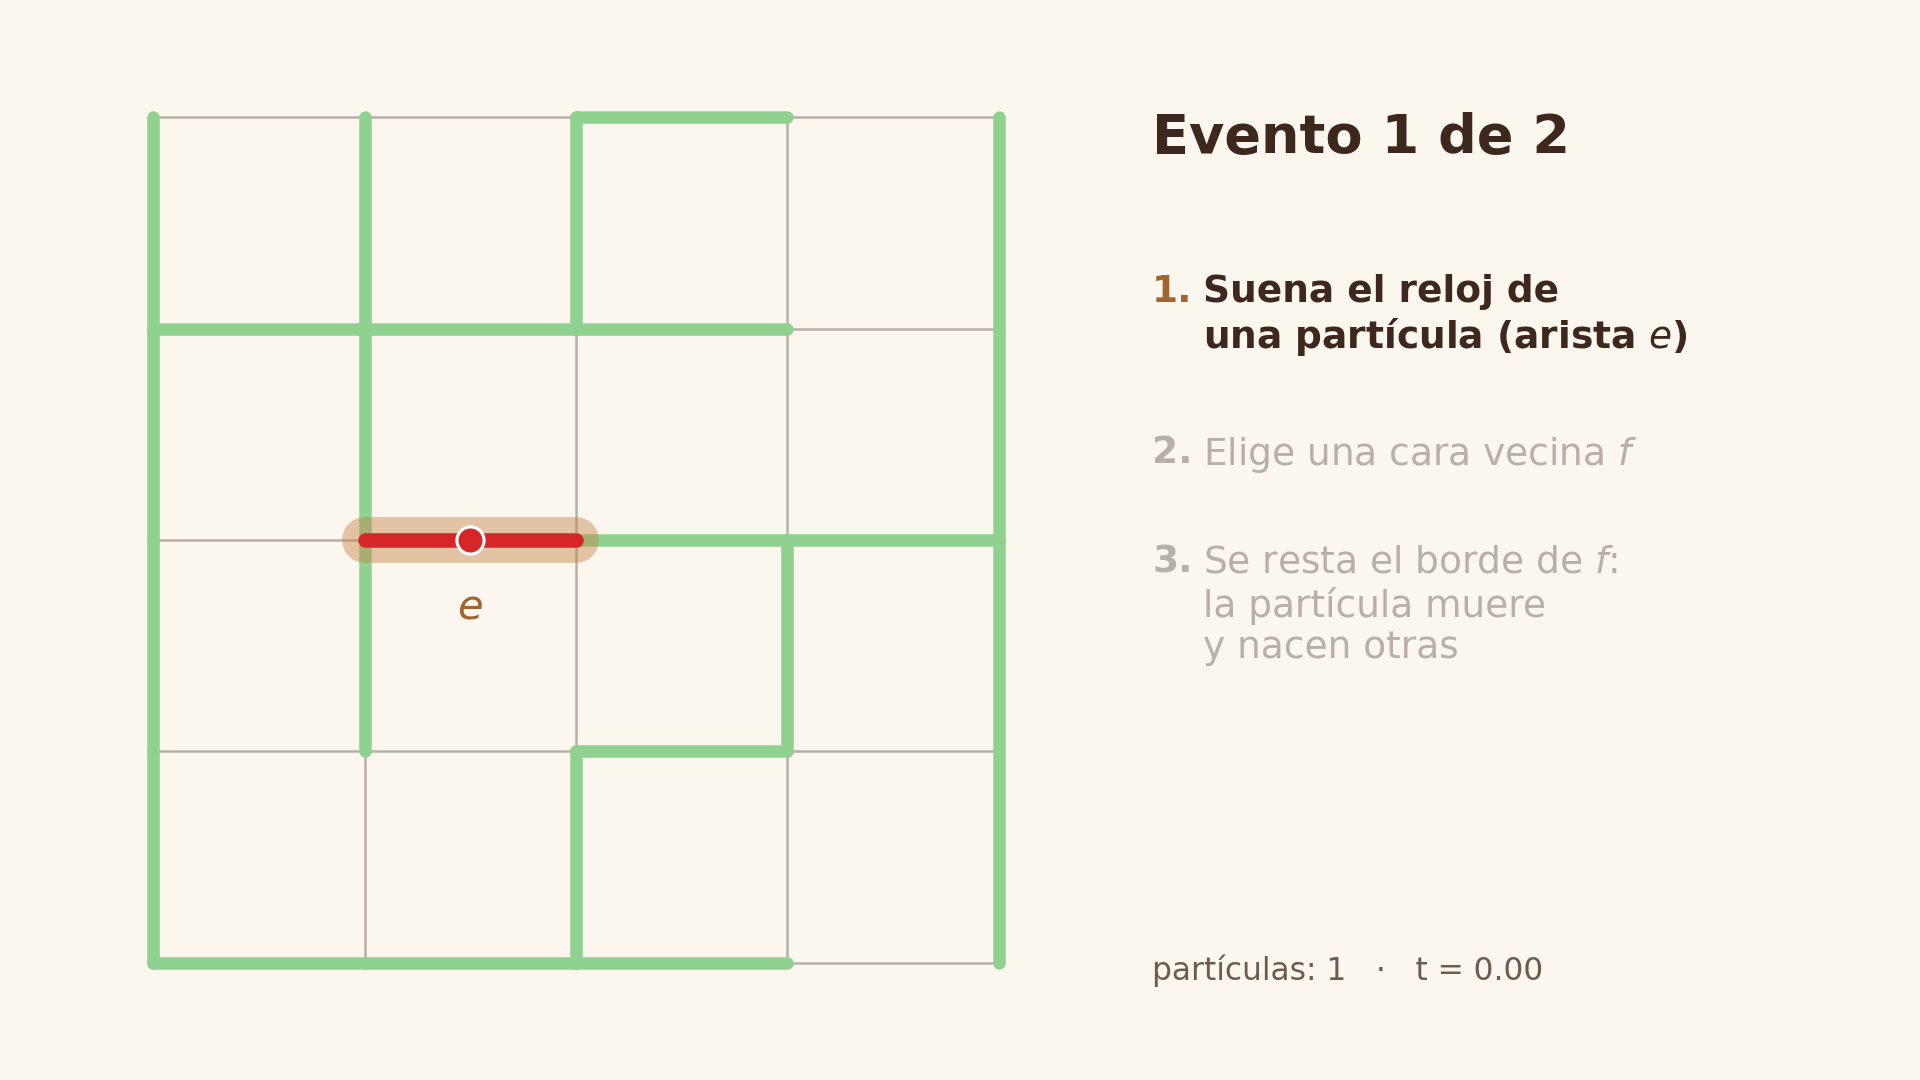
\includegraphics[height=0.84\textheight]{proceso/paso_01}
\end{frame}

\begin{frame}{Evento 1 · elige una cara}
  \centering
  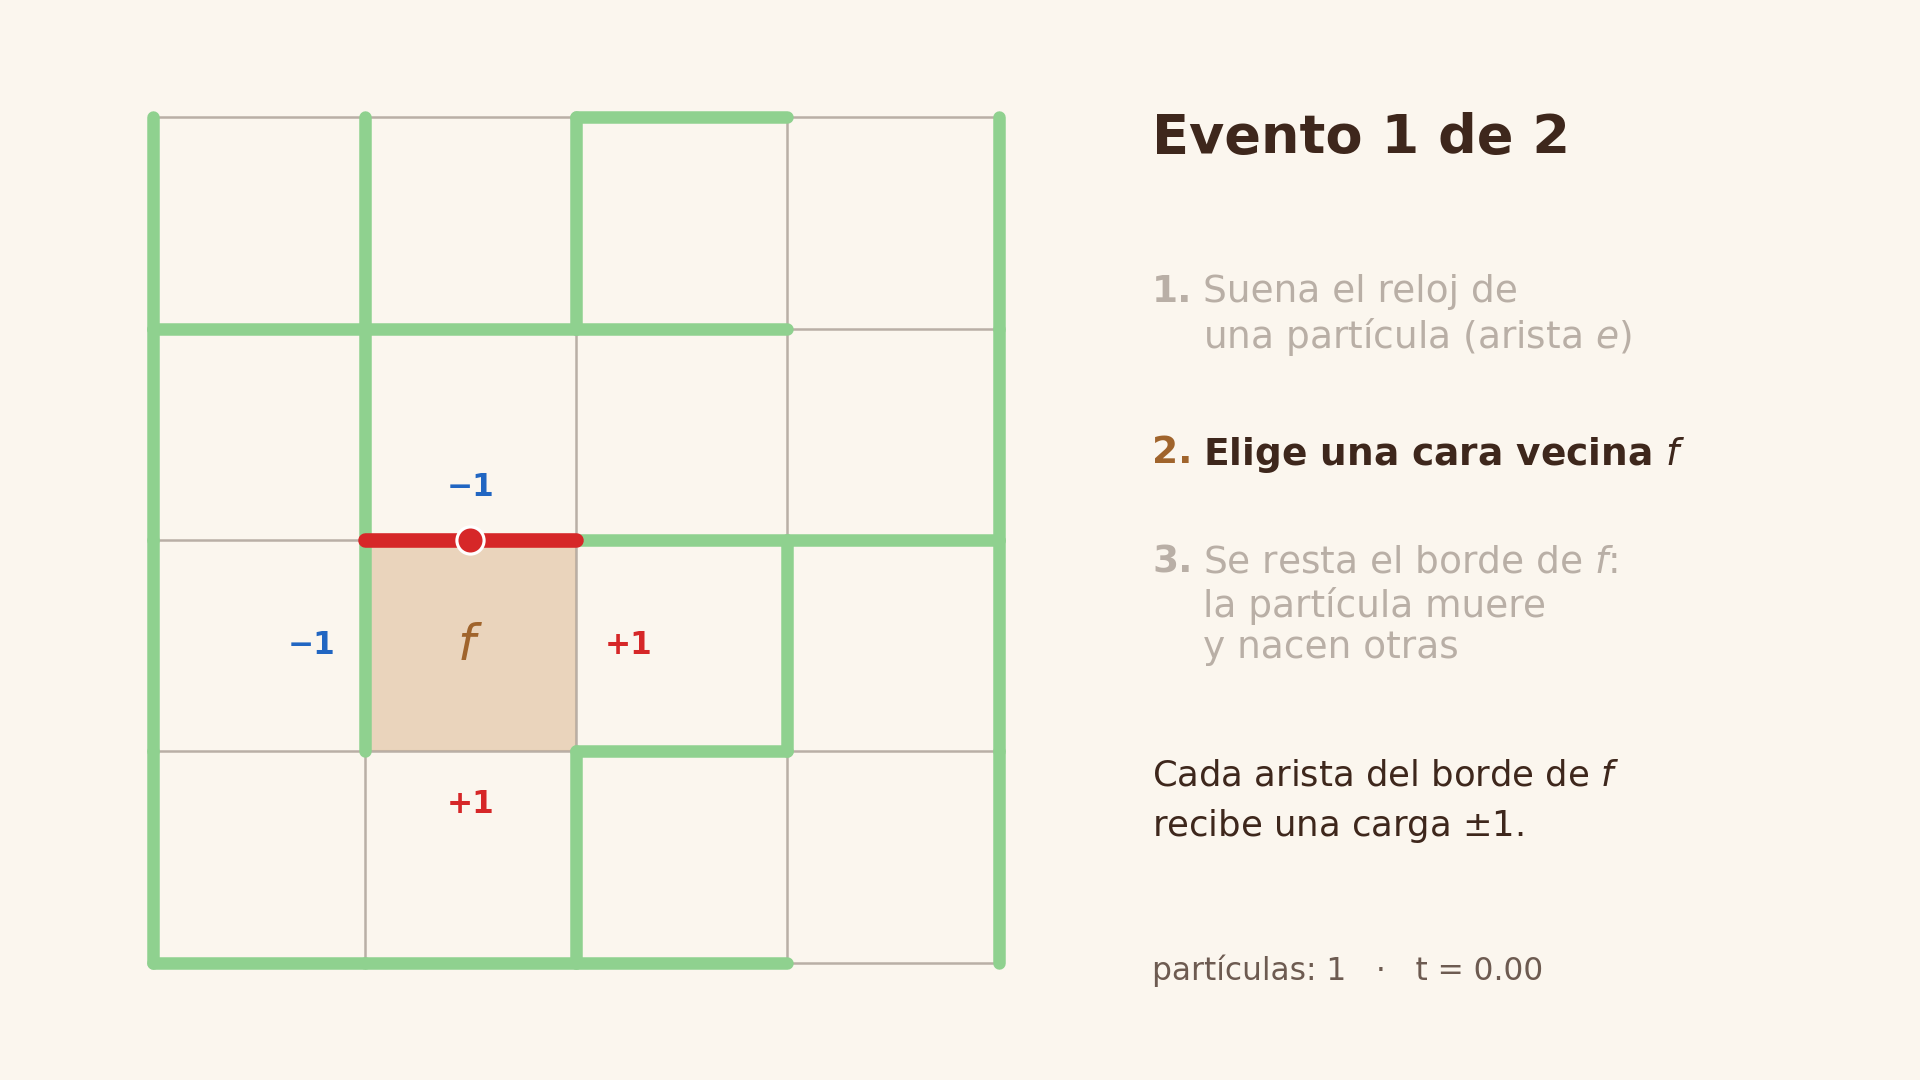
\includegraphics[height=0.84\textheight]{proceso/paso_02}
\end{frame}

\begin{frame}{Evento 1 · resultado}
  \centering
  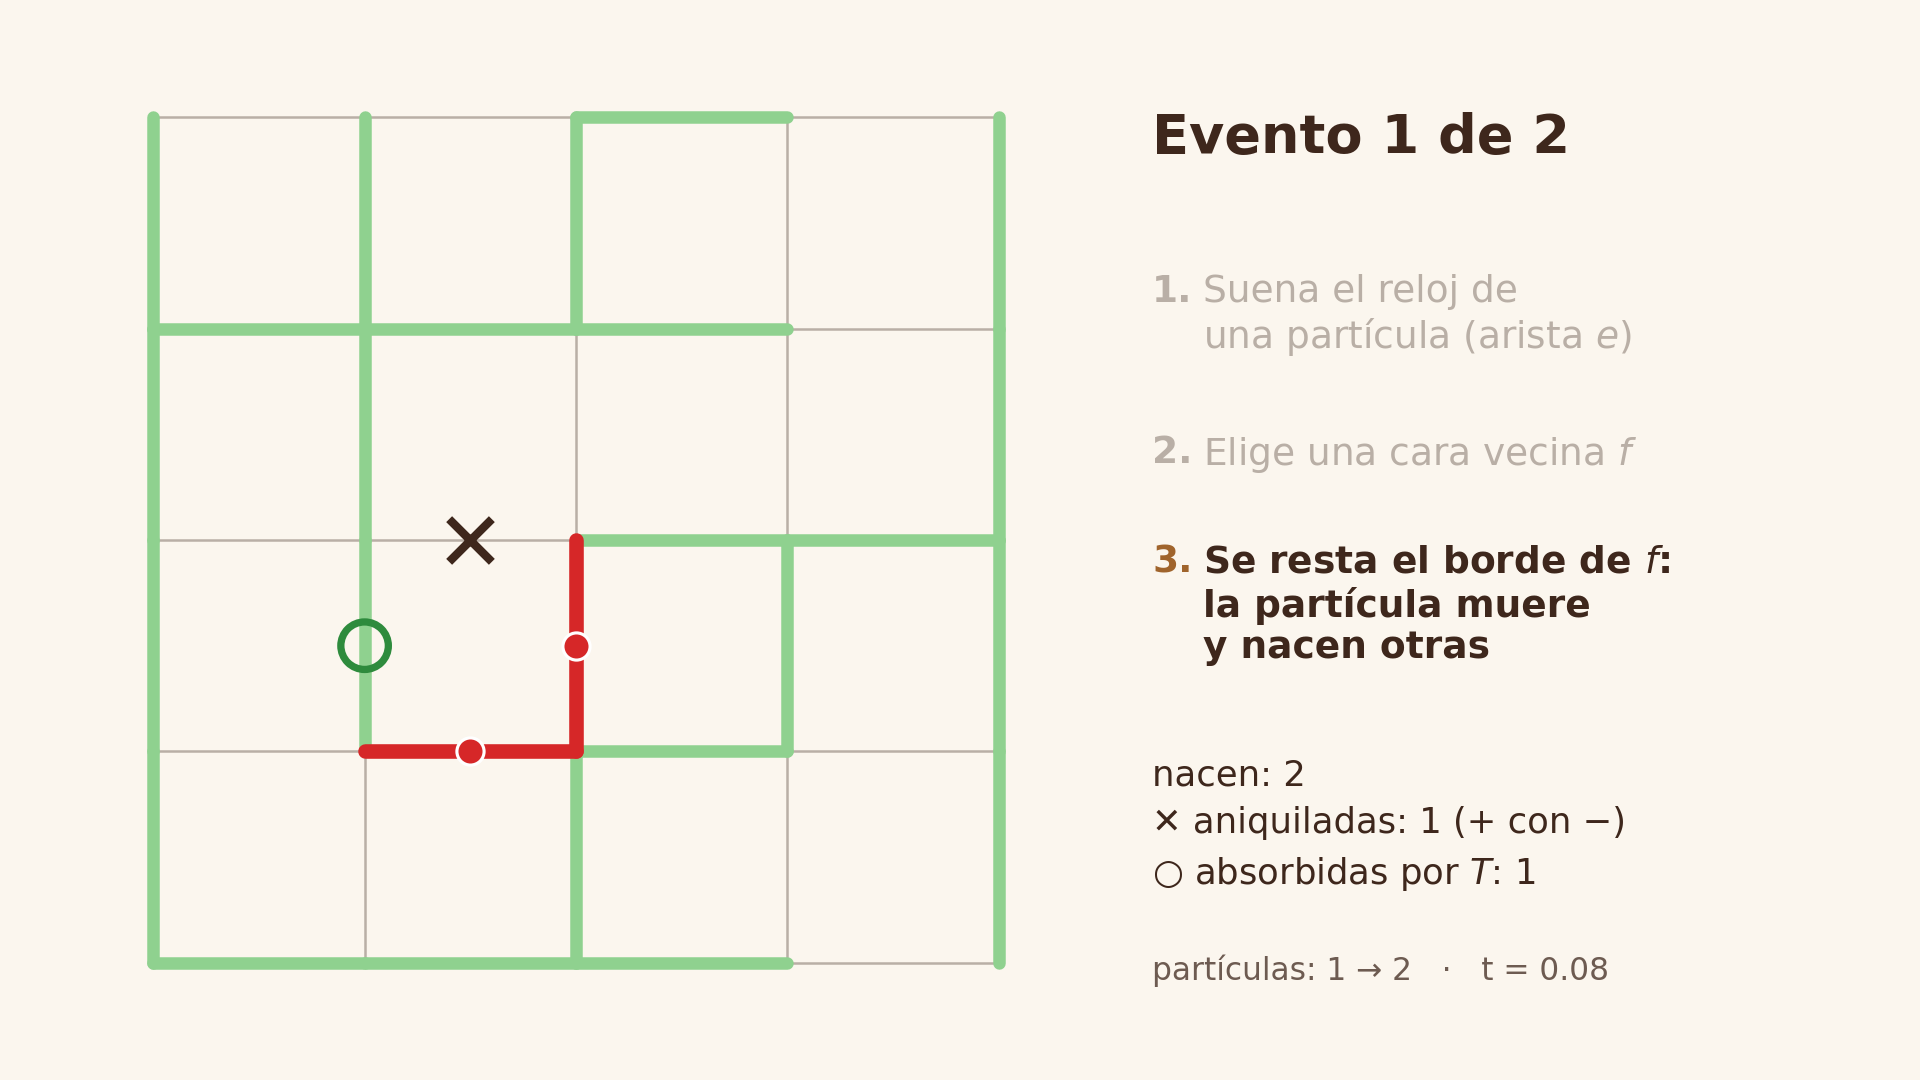
\includegraphics[height=0.84\textheight]{proceso/paso_03}
\end{frame}

\begin{frame}{Evento 2 · suena un reloj}
  \centering
  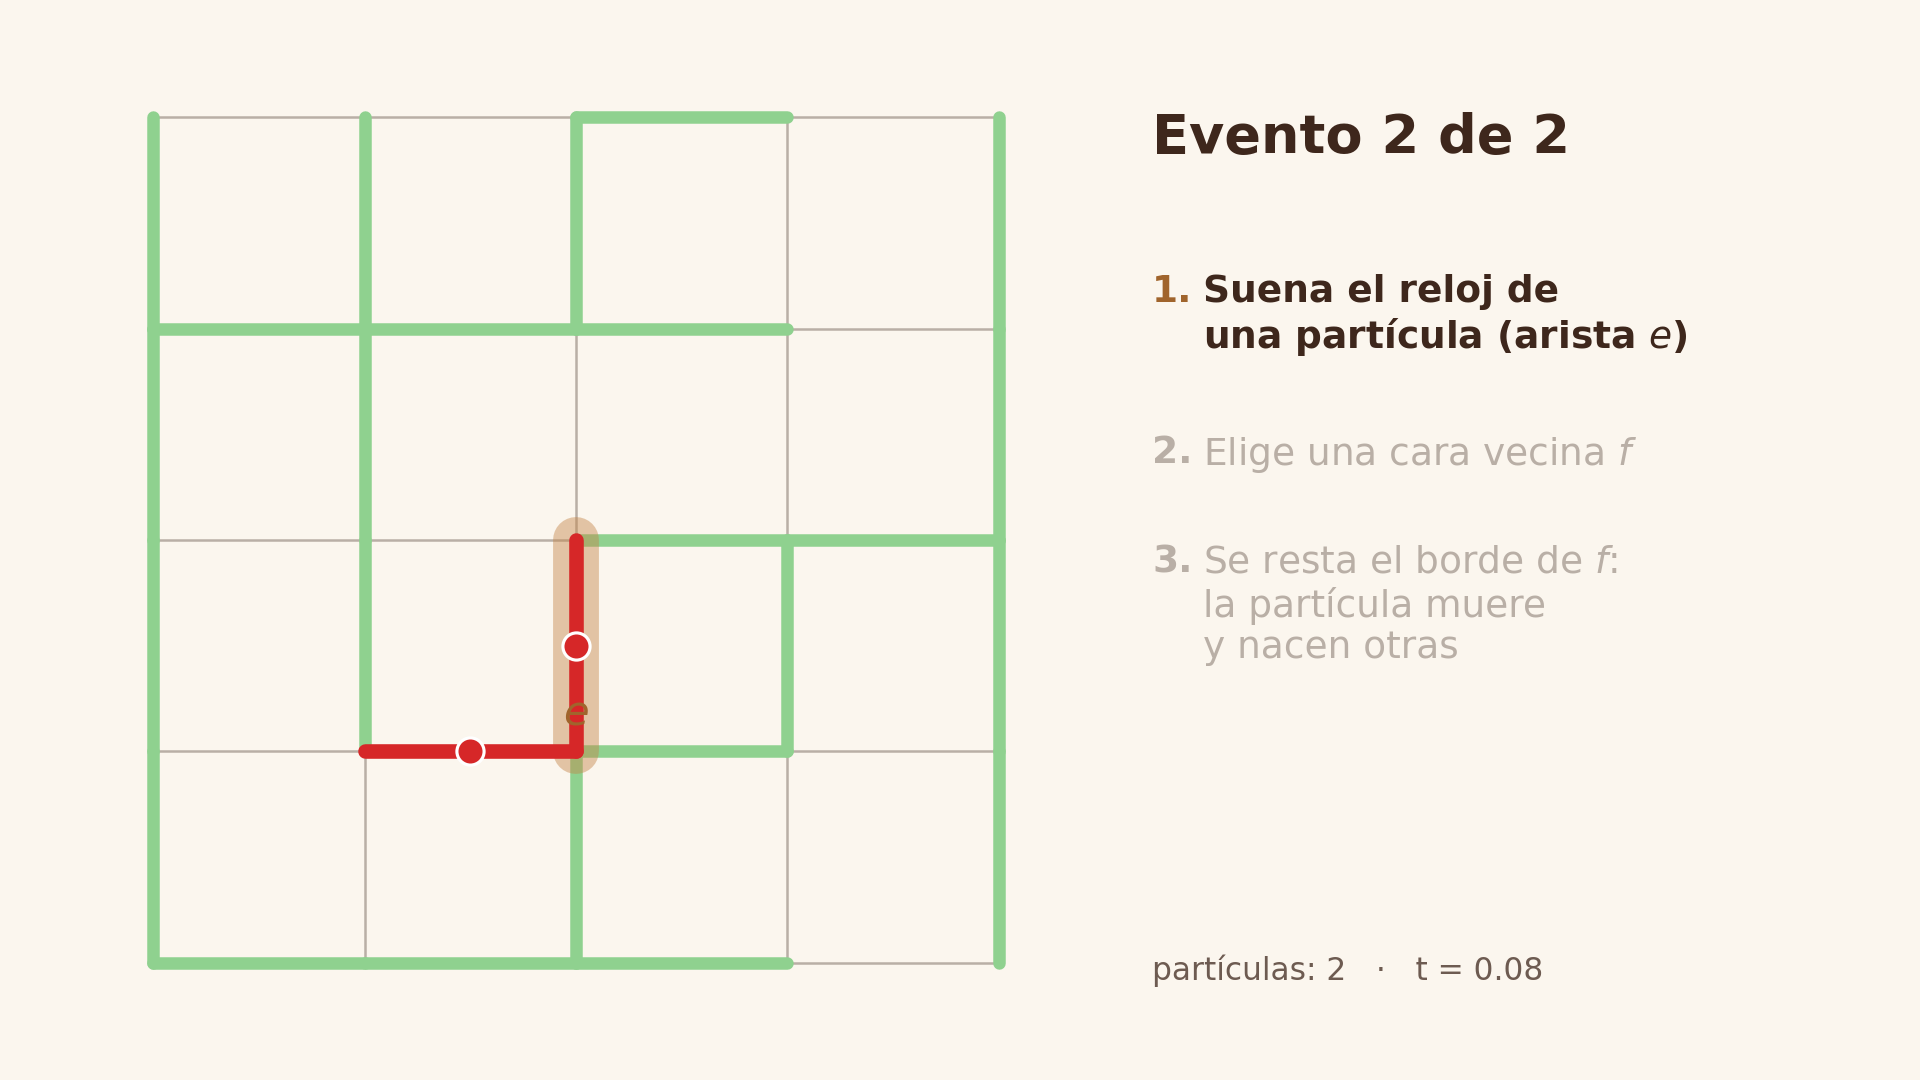
\includegraphics[height=0.84\textheight]{proceso/paso_04}
\end{frame}

\begin{frame}{Evento 2 · elige una cara}
  \centering
  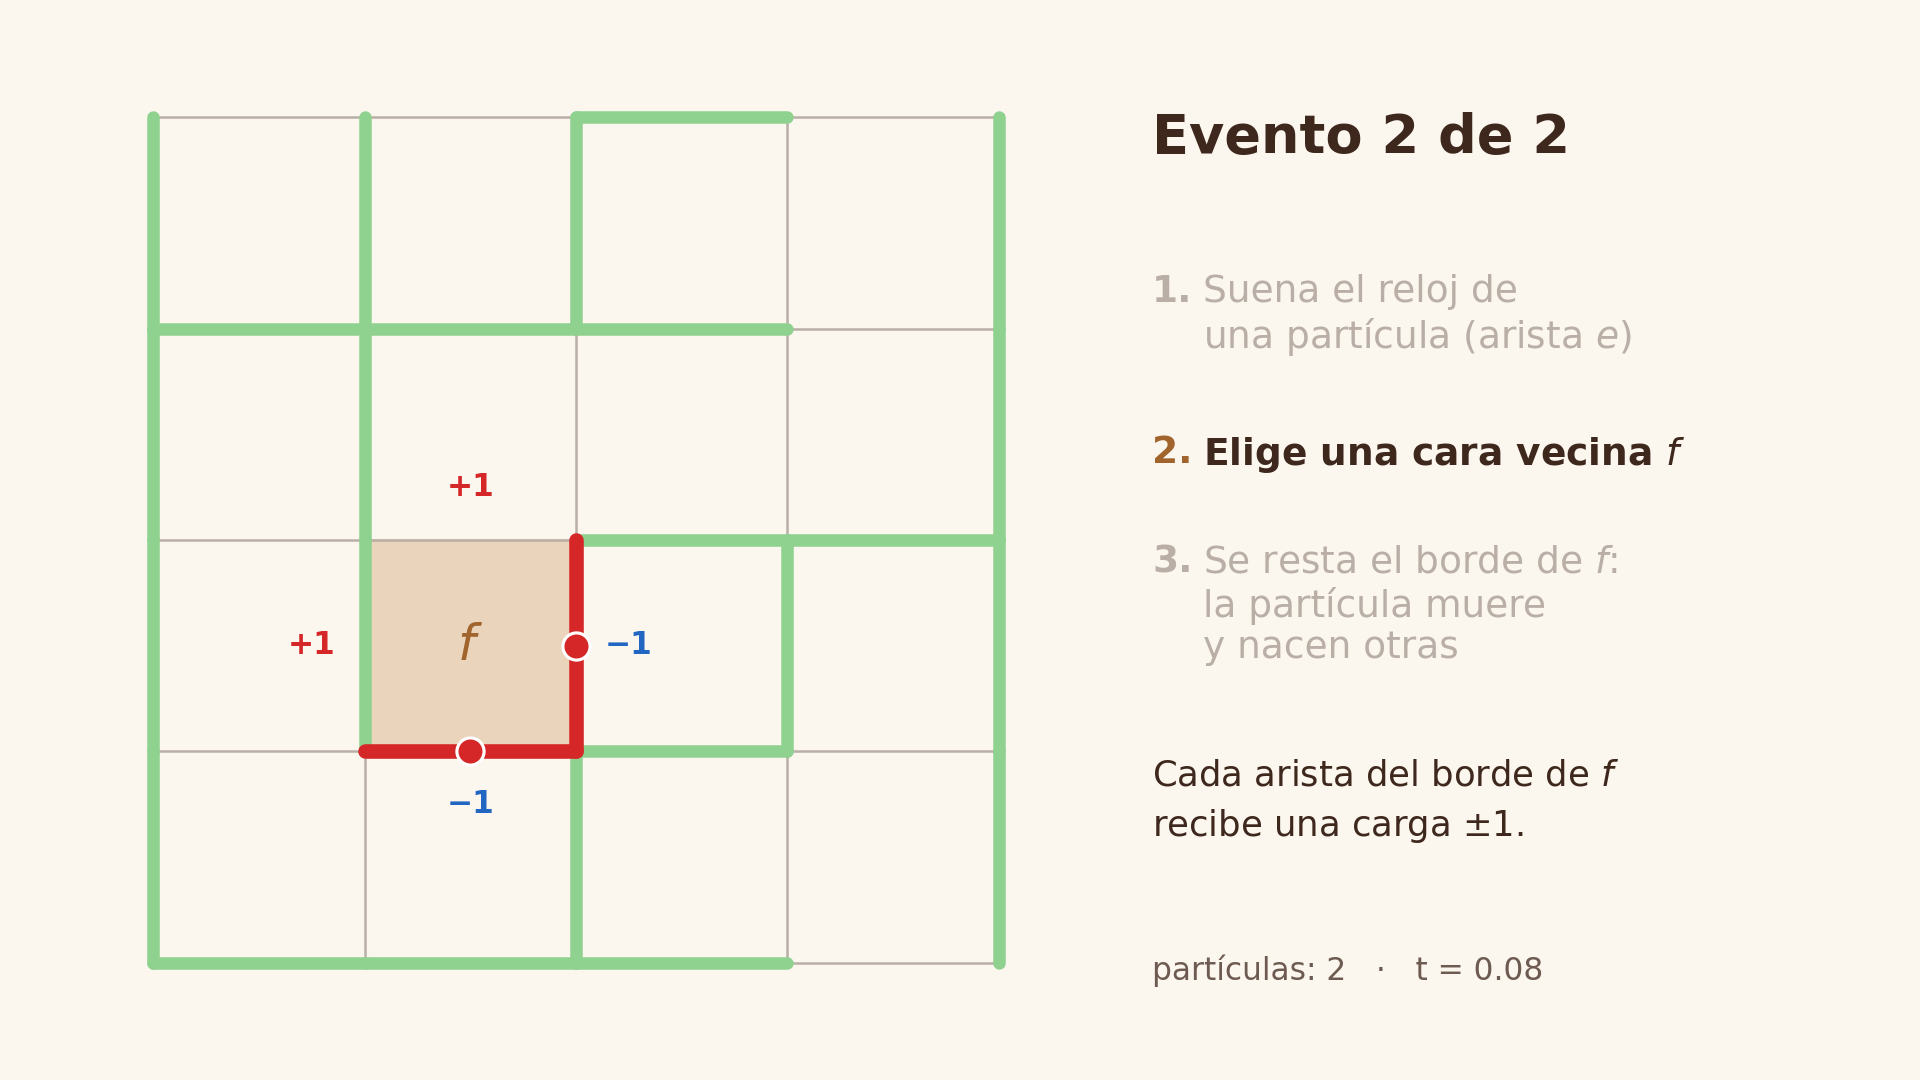
\includegraphics[height=0.84\textheight]{proceso/paso_05}
\end{frame}

\begin{frame}{Evento 2 · resultado}
  \centering
  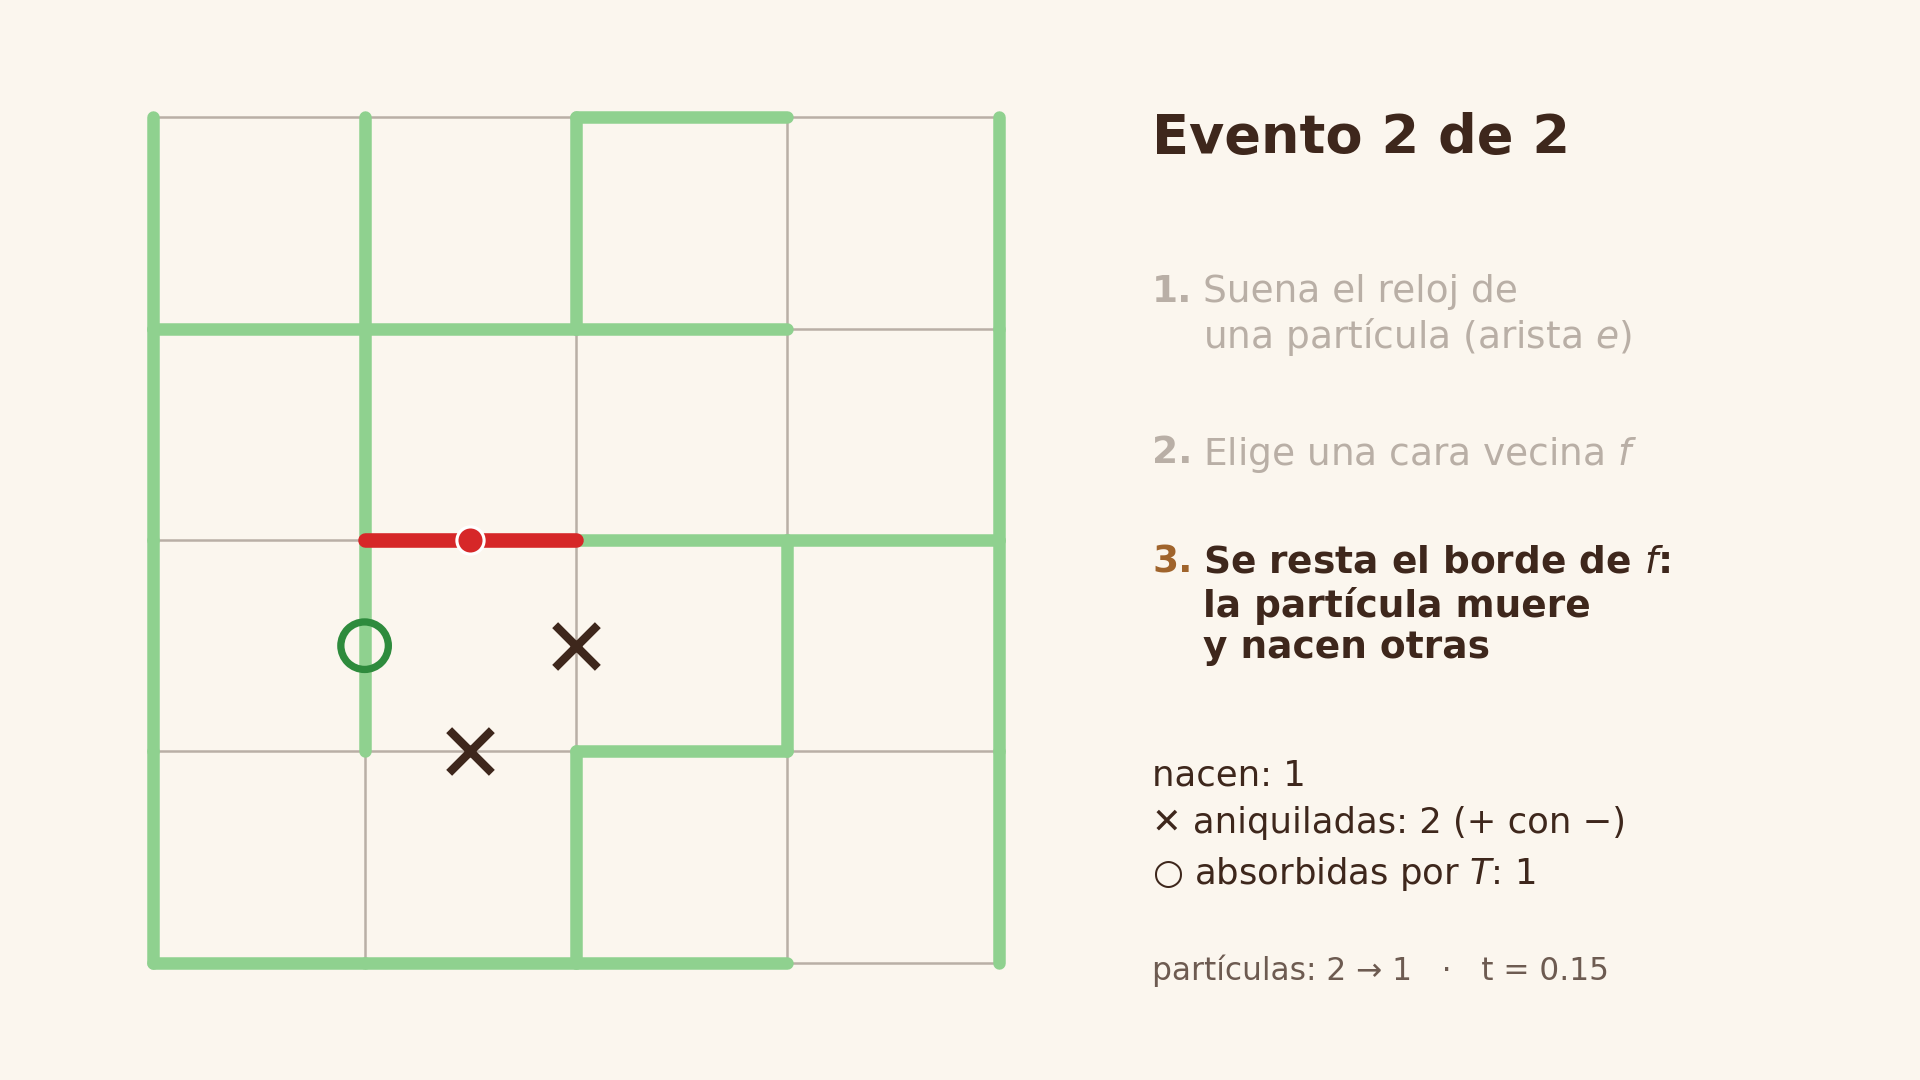
\includegraphics[height=0.84\textheight]{proceso/paso_06}
\end{frame}

\begin{frame}{¿Por qué estudiarlo?}
  % GUION (0:45): convencer.
  %  - Es la versión "de dimensión alta" de los procesos de ramificación y paseos aleatorios:
  %    en vez de vértices, aristas y caras; la geometría la da el Laplaciano de Hodge.
  %  - Compiten dos fuerzas: la ramificación (1→3) empuja a crecer, la aniquilación y la
  %    absorción a morir. ¿Quién gana? Es la pregunta clásica de la extinción.
  %  - El paper prueba que con un árbol generador se extingue, pero no dice cuándo ni qué
  %    pasa con otros conjuntos absorbentes: ahí entra la simulación.
  \begin{columns}[T]
    \begin{column}{0.31\textwidth}
      \begin{block}{Dimensión alta}
        \centering aristas y caras\\ Laplaciano de Hodge
      \end{block}
    \end{column}
    \begin{column}{0.31\textwidth}
      \begin{block}{Dos fuerzas}
        \centering ramificación $1\to3$\\ vs.\ aniquilación
      \end{block}
    \end{column}
    \begin{column}{0.31\textwidth}
      \begin{alertblock}{Pregunta abierta}
        \centering ¿cuándo y cuánto\\ tarda la extinción?
      \end{alertblock}
    \end{column}
  \end{columns}
  \vspace{5mm}
  \centering
  paper: $\;\mathcal{L}I(\theta)=-\Delta_1^{\uparrow}\theta$, \quad árbol generador $\Rightarrow$ extinción
\end{frame}

\begin{frame}{Nuestro enfoque: simulación exacta}
  % GUION (1:00): construimos un simulador exacto (Gillespie): cada (partícula, cara)
  % tiene un reloj exponencial; el mínimo es exponencial y el que suena primero es
  % proporcional a su tasa: no hay discretización del tiempo. Solo cambian 4 aristas
  % por evento (~10 µs/evento). Con muchas réplicas independientes estimamos
  % probabilidades con intervalos de Wilson. Verificamos el simulador contra la teoría
  % del paper (drift con 0.55% de error, cota de Lyapunov).
  \begin{enumerate}
    \item esperar $\;\tau\sim\mathrm{Exp}(R)$, \quad $R=\sum_e|\theta_e|\lambda_e$
    \item elegir arista $\propto|\theta_e|\lambda_e$ y cara uniforme
    \item $\theta\leftarrow\theta-c\,\partial_T f$ \quad(4 aristas)
  \end{enumerate}
  \vspace{3mm}
  \begin{columns}[T]
    \begin{column}{0.48\textwidth}
      \begin{alertblock}{Exacto}
        \centering $\min_i X_i\sim\mathrm{Exp}\big(\textstyle\sum_ir_i\big)$
      \end{alertblock}
    \end{column}
    \begin{column}{0.48\textwidth}
      \begin{block}{Miles de réplicas}
        \centering $\hat p$ + intervalos de Wilson
      \end{block}
    \end{column}
  \end{columns}
\end{frame}

% =====================================================================
%  BLOQUE 2 · RESULTADOS · ~4:15
%  Persona 1 sigue hasta "Cargas conservadas" (~1:30); luego Persona 2.
% =====================================================================

\metroset{sectionpage=progressbar}
\section{Resultados}

\begin{frame}{La dinámica}
  % GUION (0:30) [Persona 1]: mostrar el video 2D (10 partículas + árbol verde). En el
  % del lazo las partículas son el borde de una región (θ = θ0 + ∂η).
  \begin{columns}[c]
    \begin{column}{0.5\textwidth}
      \centering
      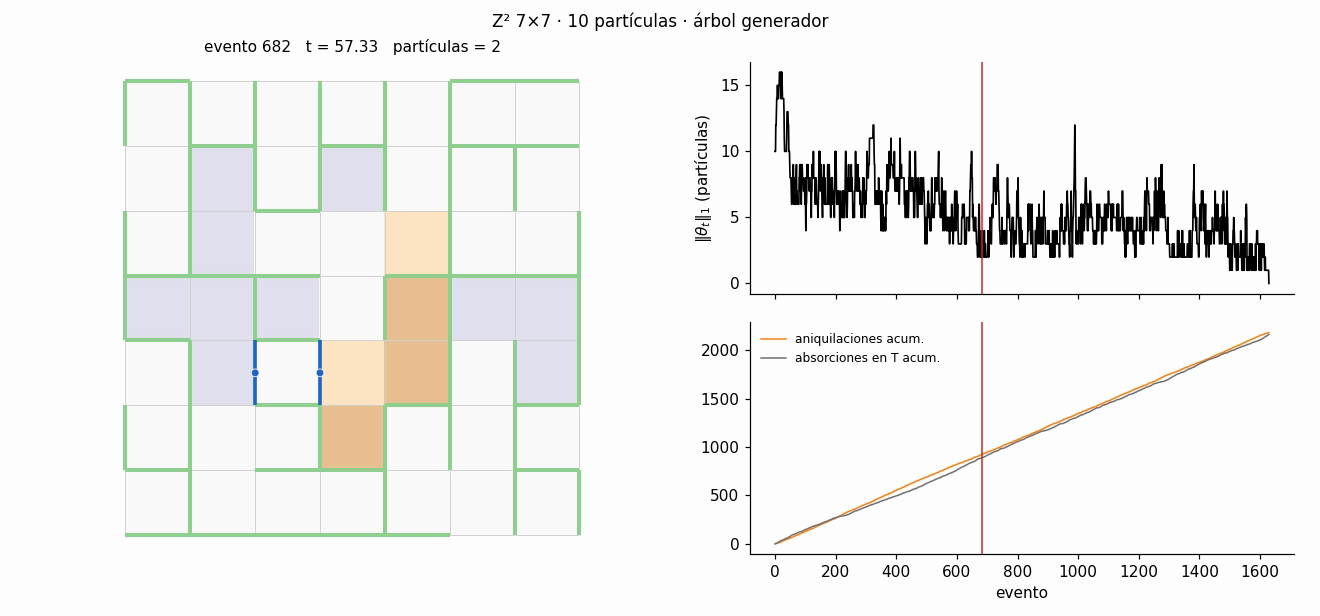
\includegraphics[width=\linewidth]{vid_z2_10particulas.png}\\
      \video{z2_10particulas_arbol.mp4}{ver video}
    \end{column}
    \begin{column}{0.5\textwidth}
      \centering
      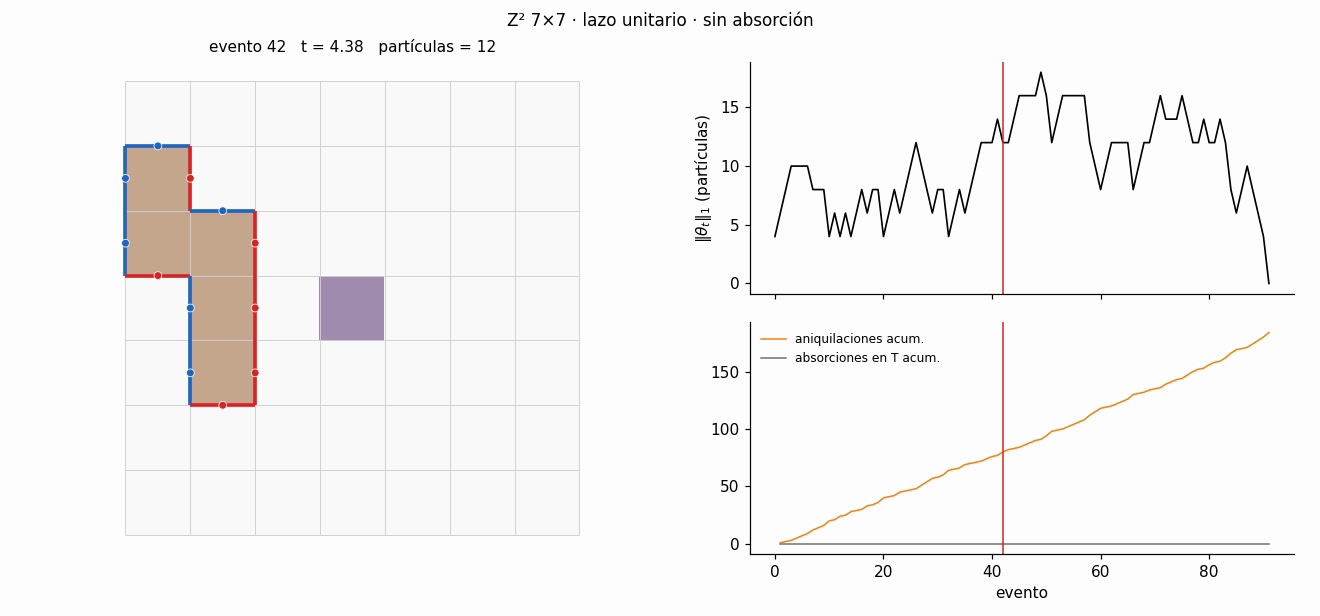
\includegraphics[width=\linewidth]{vid_z2_lazo_sin_arbol.png}\\
      \video{z2_lazo_sin_arbol.mp4}{ver video}
    \end{column}
  \end{columns}
\end{frame}

\begin{frame}{Cargas conservadas}
  % GUION (1:00) [Persona 1]: resultado principal. Para cada componente del grafo de
  % aristas absorbentes, el flujo neto se conserva. Si alguno es distinto de cero, no
  % puede extinguirse. Una partícula se extingue sii sus extremos quedan conectados por T.
  % Verificado: 2400 simulaciones, 0 errores.
  \begin{columns}[c]
    \begin{column}{0.38\textwidth}
      \centering
      \[
        Q_C=\sum_{v\in C}(\partial_1\theta)(v)
      \]
      \alert{se conserva}\\[3mm]
      $Q_C\neq0\;\Rightarrow\;$ no se extingue
    \end{column}
    \begin{column}{0.6\textwidth}
      \centering
      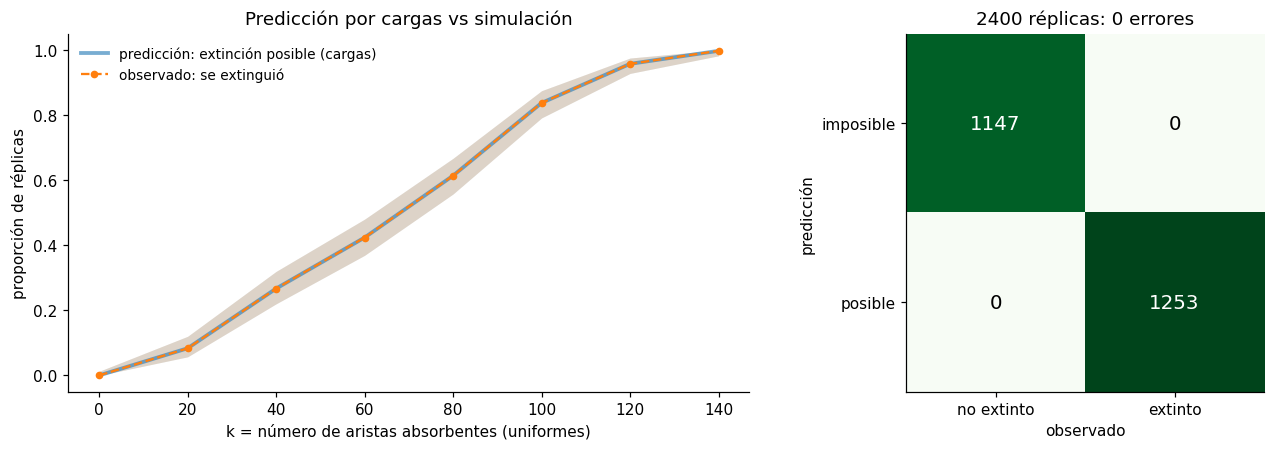
\includegraphics[width=\linewidth]{verificacion_cargas.png}
    \end{column}
  \end{columns}
\end{frame}

\begin{frame}{Extinción vs número de aristas absorbentes}
  % GUION (0:40) [Persona 2]: la probabilidad de extinción eventual se calcula EXACTA con
  % las cargas (es conectividad, tipo percolación) y crece con k. El lazo se extingue siempre.
  \centering
  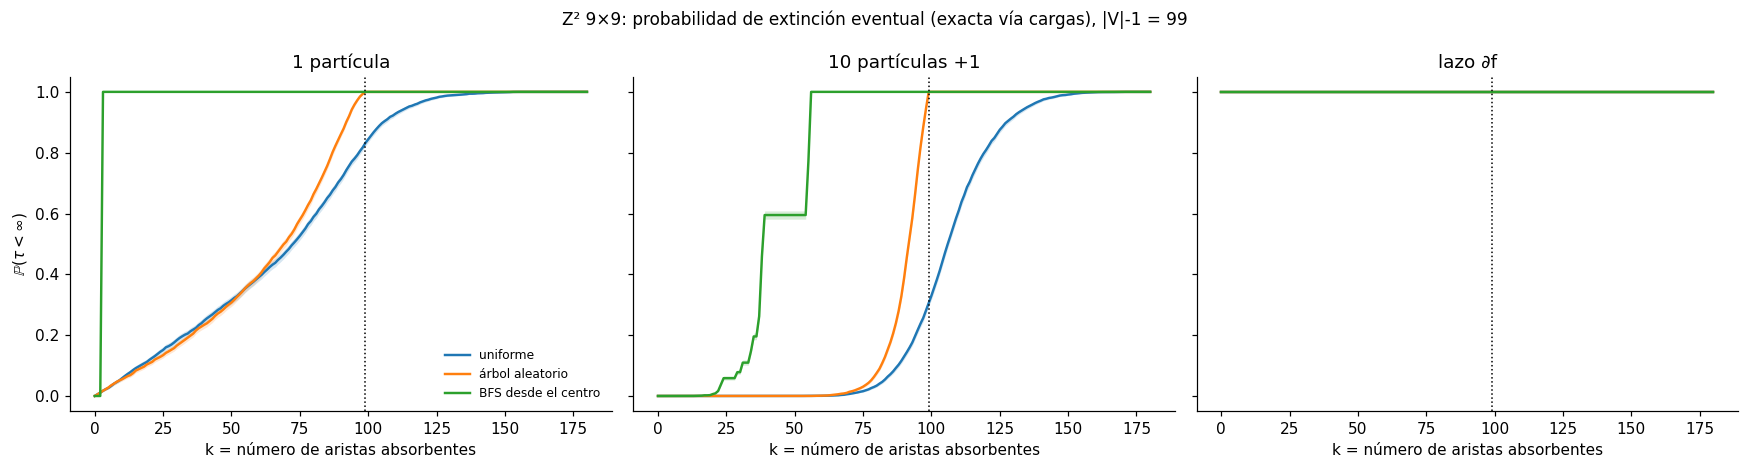
\includegraphics[width=\textwidth]{aristas_exacta.png}
\end{frame}

\begin{frame}{¿Más absorción, extinción más rápida? No siempre}
  % GUION (0:40) [Persona 2]: en tiempo finito NO es monótono: para el lazo, agregar
  % aristas absorbentes hace más lenta la extinción (1.00 → 0.94). Hipótesis: el árbol
  % corta el lazo en cadenas abiertas.
  \centering
  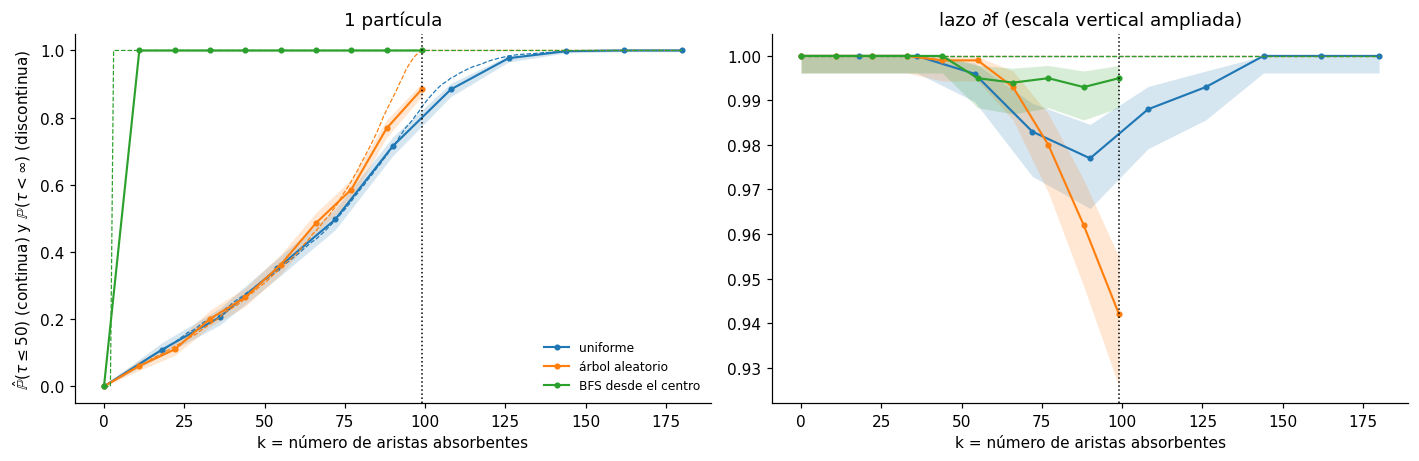
\includegraphics[width=0.9\textwidth]{aristas_tiempo_finito.png}
\end{frame}

\begin{frame}{$T$ creciendo durante la simulación}
  % GUION (0:30) [Persona 2]: una arista nueva cada m eventos. Una partícula: muere apenas
  % sus extremos se conectan (59/99 aristas). Lazo: el árbol se completa y el lazo,
  % ya cortado, sobrevive ~100 eventos más.
  \begin{columns}[c]
    \begin{column}{0.5\textwidth}
      \centering
      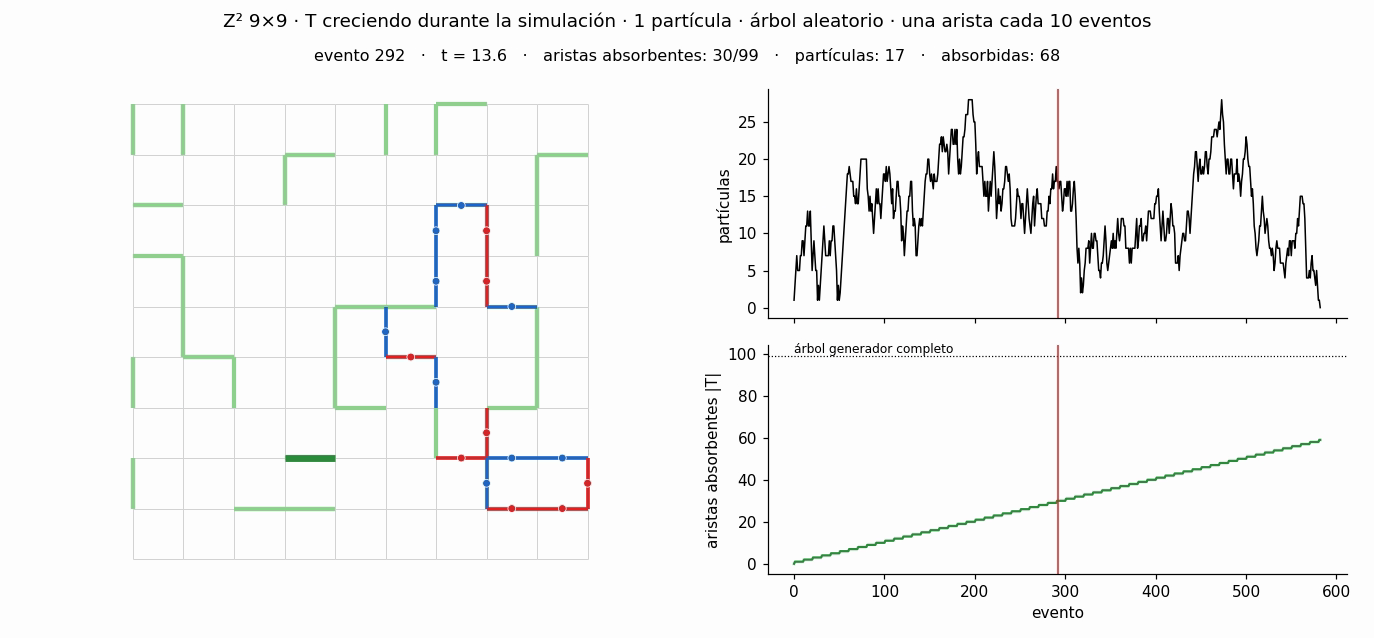
\includegraphics[width=\linewidth]{vid_T_creciente_1particula.png}\\
      \video{z2_T_creciente_1particula.mp4}{ver video}
    \end{column}
    \begin{column}{0.5\textwidth}
      \centering
      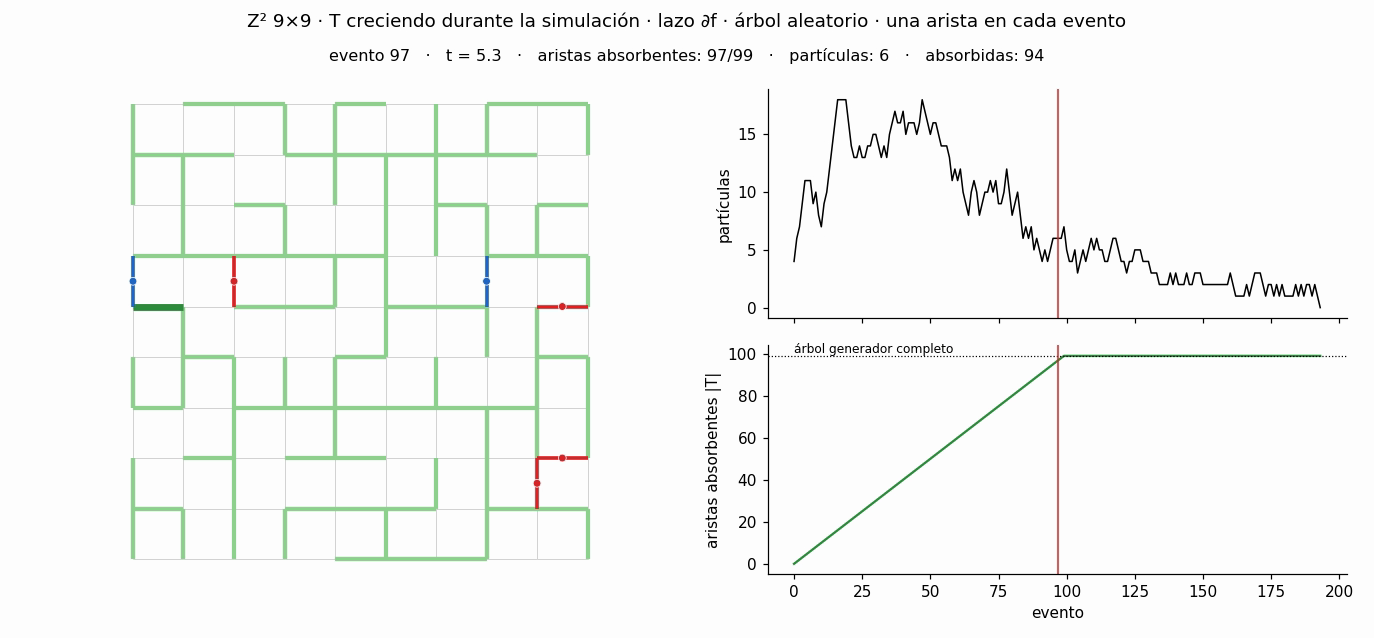
\includegraphics[width=\linewidth]{vid_T_creciente_lazo.png}\\
      \video{z2_T_creciente_lazo.mp4}{ver video}
    \end{column}
  \end{columns}
\end{frame}

\begin{frame}{En 3D: la meseta}
  % GUION (0:45) [Persona 2]: en 3D el proceso queda en una meseta cuasi-estacionaria.
  % Corrida honesta (primera semilla, sin elegir): 90 millones de eventos hasta
  % extinguirse. Desde la meseta el tiempo de extinción es ~exponencial; la caída final
  % es brusca.
  \begin{columns}[c]
    \begin{column}{0.6\textwidth}
      \centering
      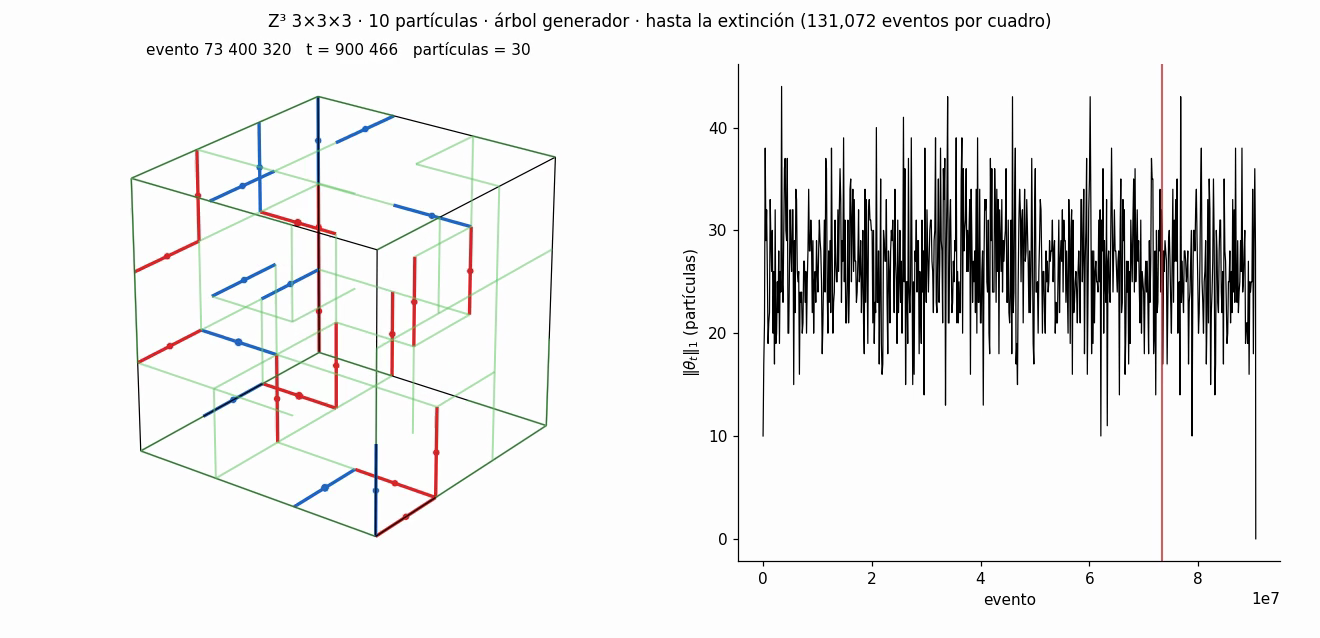
\includegraphics[width=\linewidth]{vid_z3_10particulas_extincion.png}\\
      \video{z3_10particulas_hasta_extincion.mp4}{ver video}
    \end{column}
    \begin{column}{0.38\textwidth}
      \centering
      $3\times3\times3$, sin selección\\[2mm]
      \begin{tabular}{@{}lr@{}}
        \toprule
        lazo & 23\,M \\
        10 partículas & \alert{90\,M} \\
        \bottomrule
      \end{tabular}\\[1mm]
      {\small eventos hasta la extinción}
    \end{column}
  \end{columns}
\end{frame}

% =====================================================================
%  BLOQUE 3 · CONCLUSIONES Y PASOS FUTUROS · ~2:00 · Persona 2
% =====================================================================

\section{Conclusiones y pasos futuros}

\begin{frame}{Conclusiones}
  % GUION (0:40): simulador exacto y verificado; las cargas conservadas deciden si hay
  % extinción (y la vuelven un problema de conectividad); la velocidad no es monótona;
  % en 3D aparece una meseta y la extinción tarda decenas de millones de eventos.
  \begin{enumerate}
    \item simulador \alert{exacto}, verificado contra la teoría
    \item \alert{cargas conservadas} deciden si hay extinción
    \item la \emph{velocidad} de extinción no es monótona en $T$
    \item en 3D: meseta cuasi-estacionaria
  \end{enumerate}
\end{frame}

\begin{frame}{Pasos futuros}
  % GUION (0:50):
  %  - Demostrar la hipótesis de accesibilidad (la única pieza no probada del teorema).
  %  - Conjetura: la tasa de extinción con árbol fijo es la constante de Poincaré,
  %    γ(T) ≈ c'(T) (correlación 0.95 en 40 árboles): probarla o refutarla.
  %  - Explicar la no monotonía (¿el árbol "corta" los lazos?).
  %  - Árbol generador uniforme (algoritmo de Wilson) y Fleming-Viot para estudiar la
  %    meseta en 3D sin esperar la extinción.
  \begin{itemize}
    \item demostrar la \alert{accesibilidad}
    \item conjetura: $\gamma(T)\approx c'(T)$ \quad (tasa $=$ Poincaré)
    \item explicar la no monotonía
    \item árbol uniforme (Wilson) y Fleming--Viot en 3D
  \end{itemize}
\end{frame}

\begin{frame}{Stochastic Ninja Warrior}
  % GUION (0:30): cierre. ¿Y si el conjunto absorbente se mueve? Cruz que gira y anillo
  % que oscila; 8 concursantes; cada × es una eliminación. Nadie llega a GAME OVER:
  % ramificación y eliminaciones se equilibran.
  \begin{columns}[c]
    \begin{column}{0.5\textwidth}
      \centering
      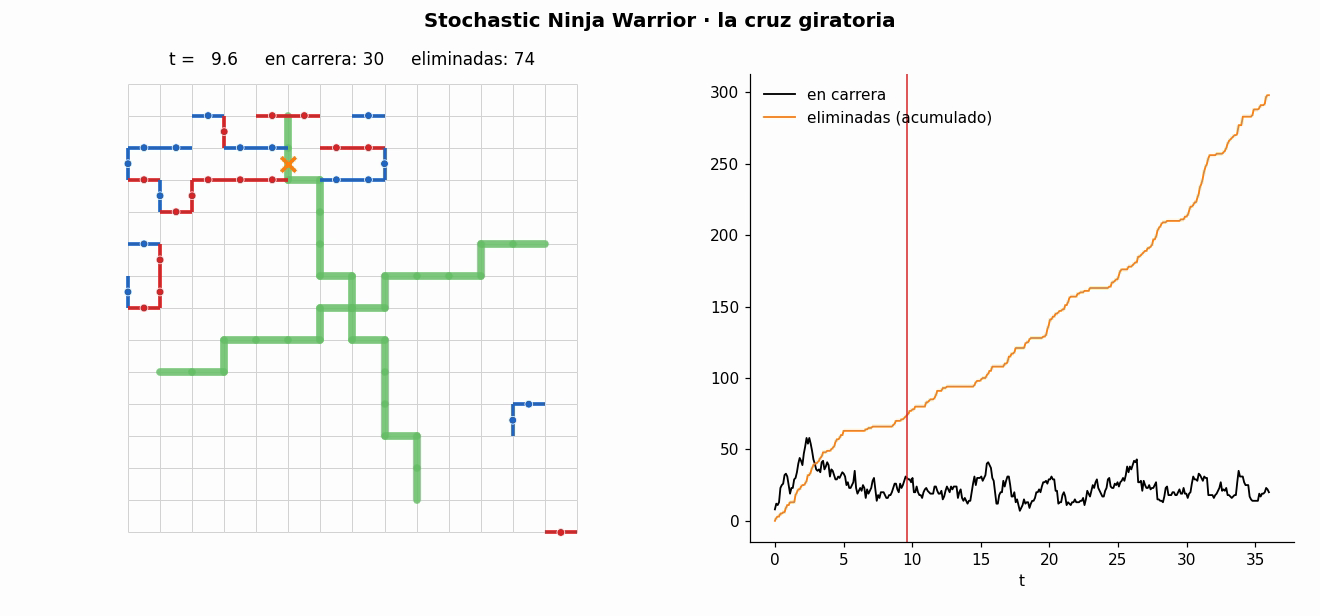
\includegraphics[width=\linewidth]{ninja_cruz.png}\\
      \video{ninja_cruz.mp4}{ver video}
    \end{column}
    \begin{column}{0.5\textwidth}
      \centering
      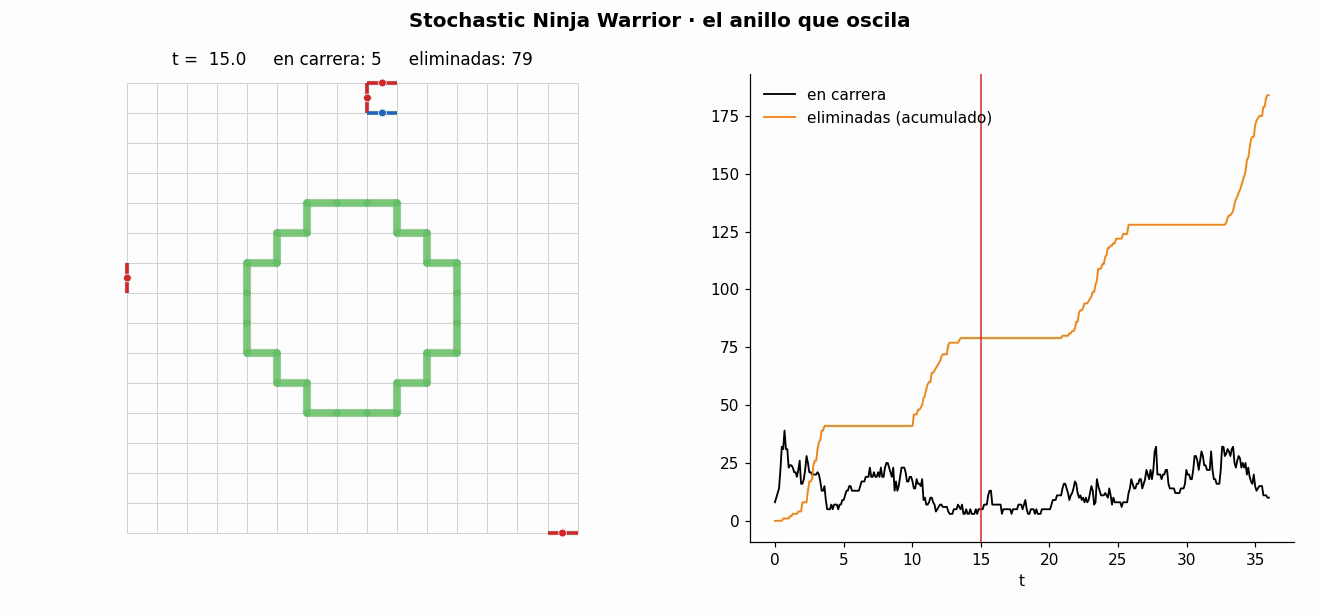
\includegraphics[width=\linewidth]{ninja_anillo.png}\\
      \video{ninja_anillo.mp4}{ver video}
    \end{column}
  \end{columns}
\end{frame}

\begin{frame}[standout]
  ¡Gracias!\\[4mm]
  {\normalsize ¿Preguntas?}\\[6mm]
  {\footnotesize \url{https://github.com/martinmaturana777/Branching-Process-Complexes}}
\end{frame}

% =====================================================================
%  RESPALDO (no se presenta; solo para preguntas)
% =====================================================================
\appendix

\begin{frame}{Respaldo: precisión de las estimaciones}
  % GUION: proporción de réplicas, insesgada; cortar en t* no sesga; Wilson funciona
  % aunque p̂ sea 0 o 1. Error estándar ≈ mitad del semiancho.
  \begin{columns}[c]
    \begin{column}{0.5\textwidth}
      \centering
      \[
        \hat p=\frac{\#\{\text{réplicas en que ocurre}\}}{R}
      \]
      intervalos de \alert{Wilson}
    \end{column}
    \begin{column}{0.45\textwidth}
      \centering
      \begin{tabular}{@{}rr@{}}
        \toprule
        réplicas & IC 95\,\% \\
        \midrule
        300 & $\pm$5.7\,\% \\
        1000 & $\pm$3.1\,\% \\
        5000 & $\pm$1.4\,\% \\
        \bottomrule
      \end{tabular}
    \end{column}
  \end{columns}
\end{frame}

\begin{frame}{Respaldo: tasa de extinción y constante de Poincaré}
  % GUION: con el árbol fijo, P(τ>t) ≈ C e^{-γ t}; γ no depende de la condición inicial;
  % en 40 árboles γ(T) ≈ c'(T) con correlación 0.95.
  \centering
  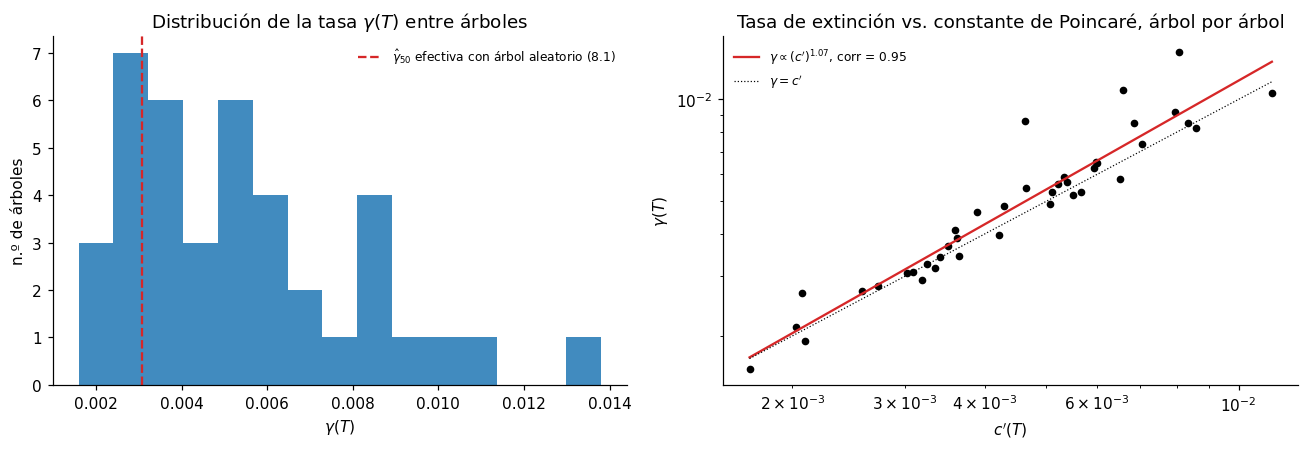
\includegraphics[width=0.9\textwidth]{ext_gamma_poincare.png}
\end{frame}

\begin{frame}{Respaldo: $T$ creciente, promedios}
  % GUION: una partícula: crecer rápido acelera la extinción (E[τ] 69 vs 432);
  % lazo: lo contrario (9.7 vs 1.1).
  \centering
  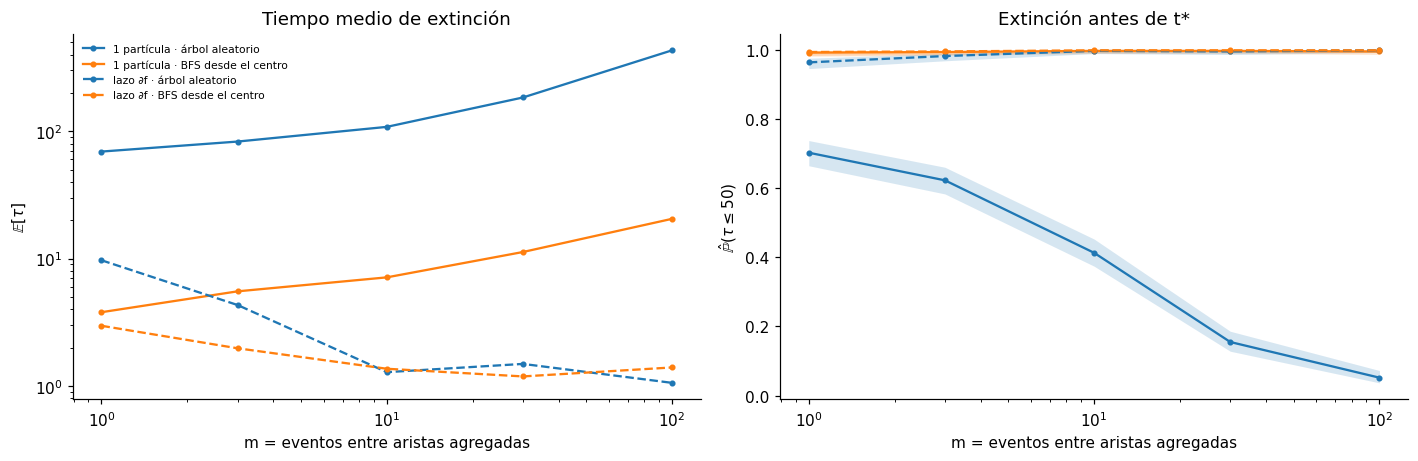
\includegraphics[width=0.9\textwidth]{aristas_dinamico.png}
\end{frame}

\end{document}
